\chapter{Ramping parameter under the random graph model} % (fold)
\label{cha:ramping_parameter_under_the_random_graph_model}

Previous work~\cite{Sindel:2009vd} provided a connection between the clustered structure of a graph and an interpretation of concentration risk.
The methodology presented by the authors considered the effects of removing edges with weight under given a varying threshold on the community structure of a fully connected obligor-correlation matrix.
In particular, by computing the variation of the component structure of the graph, the authors have shown how to analyse concrete credit portfolios and identify sets of highly connect assets.


This thesis builds upon the aforementioned model and aims at describing the expected behaviour of the ramping parameter model for theoretical graph generation models.
In this chapter, we focus on the random graph model, a well understood theoretical graph model, described in section~\vref{sec:random_graph_model}.

In particular, it tries to describe the expected behaviour of the curve designed by the~\cite{Sindel:2009vd} the problem from the perspective of having
large, idealized portfolios 
and a random graph model that generates them.





\section{The ramping parameter model} % (fold)
\label{sec:the_ramping_parameter_model}


The approach proposed by~\cite{Sindel:2009vd} for quantifying the concentration risk of a loan portfolio works can be summarized as follows:
\begin{itemize}
	\item The mutual dependency between the obligors in a portfolio is represented by a matrix $\rho_{ij}$. This matrix is symmetric, the values $\rho_{ij} \in [0,1]$, and it will be called correlation matrix throughout the remainder of this document.
	\item A so-called ramping parameter $\ramp \in [0,1]$ is used to define the effective correlation matrix $\rho_{ij}(\ramp)$ given the value of this  parameter:
	\begin{equation}
	\rho_{ij}(\ramp) = 
		\begin{cases}
		1 \text{ if } \rho_{ij} \ge \ramp,\\
		0 \text{ otherwise}.
		\end{cases}
	\end{equation}
	At $\ramp = 0$, the effective matrix will contain all connections in the original matrix. At $\ramp = 1$, all obligors in the effective matrix will be disconnected.
	
	\item The exposure-dependence is taken into account by computing the “effective” exposure for every value of $\ramp$.
\end{itemize}

To properly account for the Concentration Risk we compute the ratio $R(ρ∗)$ of the maximum of all exposures of all identified connected components $C_k$ and the total exposure of the portfolio
of the portfolio and $j$ runs over all loans within the connected component $C_k$.
\begin{figure}[tb]
	\centering
	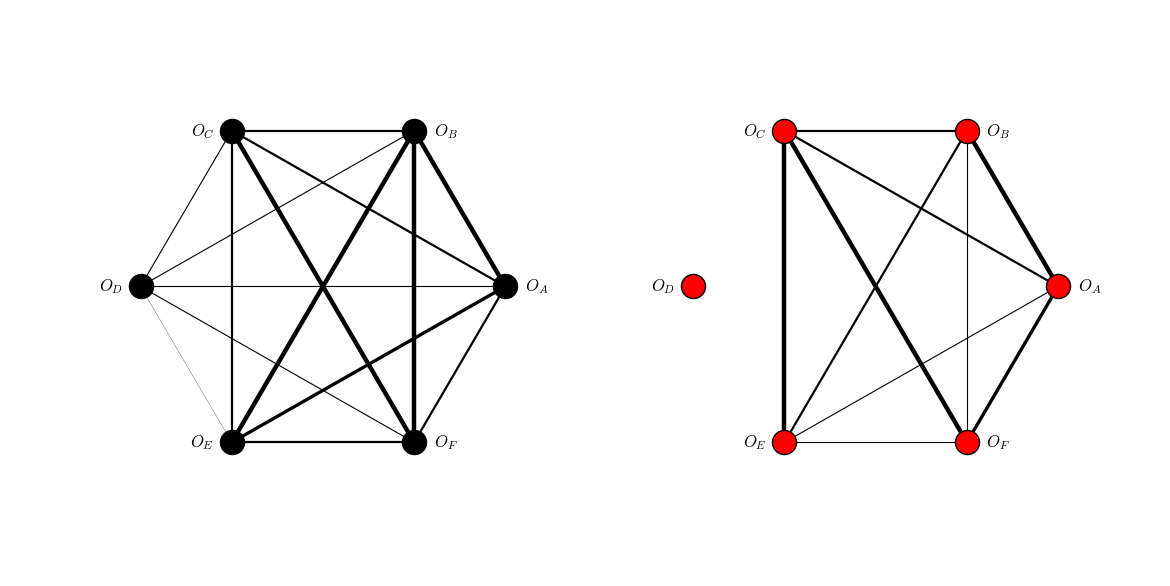
\includegraphics[scale=0.5]{figures/ramping_parameter_example.png}
	\caption{
Stylized portfolio of six obligors (A, B, C, D, E, and F).
The relative strength of the inter-obligor connections $\rho_{ij}$ is illustrated by the line-width.
In the left figure, the interdependency between customer $D$ and the other customers is rather small.
Additional to the individual inter-customer correlation each customer also has an individual obligation (symbolized by the differently coloured circles), indicated as $O_i$, $i \in \{A, B, C, D, E, F \}$.
Both the obligation of the individual customer $O_i$ and the inter-customer correlations $\rho_{ij}$ are required to compute the Concentration Risk as suggested by our measure.
For a particular value of the correlation strength obligor D becomes independent from all other obligors of the portfolio.
	}
	\label{fig:6_pf_ramping}
\end{figure}

% Formally, we define 

 
% Unnumbered theorem-like environments are also possible.
 
 
% And the next is a somewhat informal definition
 
\begin{definition}{Portfolio}
A credit portfolio is a tuple $(O, \hat{\rho})$, where $O$ is a set of $n$ exposures from $n$ different obligors and $\hat{\rho}$ an $n \times n$ matrix.
The $\rmat$ matrix represents the interdependency or correlation between each obligor $i$, and each element $\rij \in [0,1]$.
\end{definition}

\begin{remark}
Throughout this work, the matrix $\rmat$ is symmetric, so that $\forall i,j \rij = \rho_{ji}$
\end{remark}

The algorithm is described in~\ref{algo:ramping_parameter}.

\begin{algorithm}
\label{algo:ramping}
\caption{Ramping parameter algorithm~\label{algo:ramping_parameter}}
\State $\ramp \gets 0$
\State $w$ \gets \textrm{order $O_{ij}$}

\State $\epsilon\gets \min\{w_{ij}\}$

% 1. We systematically increase the ramping parameter ρ∗ from 0 to 1 with a suffi- ciently small step size.
\For{$\ramp$ \in [0,1]}

	$M \gets \textrm{compute the obligor correlation matrix as shown in eq~\ref{}}$

	$R(\rho_*) \gets \max_{C_k} \left(  \frac{\sum_{j\in C_k} \textrm{EAD}_j}{\sum_i \textrm{EAD}_i}  \right)$

\EndFor
\end{algorithm}

2. For each value of ρ∗ we compute the effective (inter) obligor-correlation matrix as shown in Eq. 3.2.
3. We compute the number of connected components and the corresponding obli- gation in each component of the graph for every value of ρ∗.4
4. To properly account for the Concentration Risk we compute the ratio R(ρ∗) of the maximum of all exposures of all identified connected components Ck and the total exposure of the portfolio
of the portfolio and j runs over all loans within the connected component Ck.

In Eq. (3.3) i runs over all loans of the portfolio, i EADi is the total obligation
Note that R(ρ∗) describes the risk of a portfolio associated with the default of its biggest clump for a given ρ∗. The risk related to a correlated default of the two biggest clumps - which has a very small probability - is not included in equation (3.3). Of course one could account for such scenarios in R(ρ∗) as well by adjusting formula (3.3). As correlated defaults are exponentially suppressed we do not incorporate them in


% section the_ramping_parameter_model (end)

\section{Ramping parameter under random graph model} % (fold)
\label{sec:ramping_parameter_under_random_graph_model}


In this chapter, we will be considering random graphs generated by the 

We will not be considering individual instances of graphs, but rather the population effects on them.



assumption:
weights are uniformly distributed and independent
exposure on nodes is independently distributed from the weights of the vertices


\begin{figure}[tb]
	\centering
	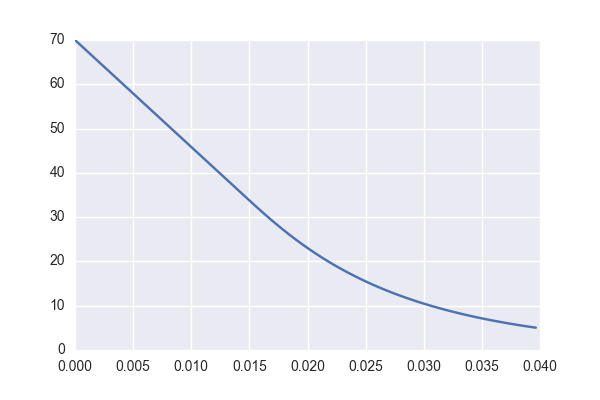
\includegraphics[]{figures/gnp_number_components.png}
	\caption{Number of components as a function of the probability $p$ of the $G(n,p)$ model.}
	\label{fig:figure1}
\end{figure}


\begin{itemize}
	\item The variation of the ramping parameter is equivalent to having random graphs generated with different $p$ probabilities.
\end{itemize}


describe the phase transition


describe the size of the components

% section ramping_parameter_under_random_graph_model (end)

% chapter ramping_parameter_under_the_random_graph_model (end)